\documentclass[]{article}
\usepackage[left=1in,top=1in,right=1in,bottom=1in]{geometry}


%%%% more monte %%%%
% thispagestyle{empty}
% https://stackoverflow.com/questions/2166557/how-to-hide-the-page-number-in-latex-on-first-page-of-a-chapter
\usepackage{color}
% \usepackage[table]{xcolor} % are they using color?

% \definecolor{WSU.crimson}{HTML}{981e32}
% \definecolor{WSU.gray}{HTML}{5e6a71}

% \definecolor{shadecolor}{RGB}{248,248,248}
\definecolor{WSU.crimson}{RGB}{152,30,50} % use http://colors.mshaffer.com to convert from 981e32
\definecolor{WSU.gray}{RGB}{94,106,113}

%%%%%%%%%%%%%%%%%%%%%%%%%%%%

\newcommand*{\authorfont}{\fontfamily{phv}\selectfont}
\usepackage{lmodern}


  \usepackage[T1]{fontenc}
  \usepackage[utf8]{inputenc}




\usepackage{abstract}
\renewcommand{\abstractname}{}    % clear the title
\renewcommand{\absnamepos}{empty} % originally center

\renewenvironment{abstract}
 {{%
    \setlength{\leftmargin}{0mm}
    \setlength{\rightmargin}{\leftmargin}%
  }%
  \relax}
 {\endlist}

\makeatletter
\def\@maketitle{%
  \pagestyle{empty}
  \newpage
%  \null
%  \vskip 2em%
%  \begin{center}%
  \let \footnote \thanks
    {\fontsize{18}{20}\selectfont\raggedright  \setlength{\parindent}{0pt} \@title \par}%
}
%\fi
\makeatother






\usepackage{color}
\usepackage{fancyvrb}
\newcommand{\VerbBar}{|}
\newcommand{\VERB}{\Verb[commandchars=\\\{\}]}
\DefineVerbatimEnvironment{Highlighting}{Verbatim}{commandchars=\\\{\}}
% Add ',fontsize=\small' for more characters per line
\usepackage{framed}
\definecolor{shadecolor}{RGB}{248,248,248}
\newenvironment{Shaded}{\begin{snugshade}}{\end{snugshade}}
\newcommand{\AlertTok}[1]{\textcolor[rgb]{0.94,0.16,0.16}{#1}}
\newcommand{\AnnotationTok}[1]{\textcolor[rgb]{0.56,0.35,0.01}{\textbf{\textit{#1}}}}
\newcommand{\AttributeTok}[1]{\textcolor[rgb]{0.77,0.63,0.00}{#1}}
\newcommand{\BaseNTok}[1]{\textcolor[rgb]{0.00,0.00,0.81}{#1}}
\newcommand{\BuiltInTok}[1]{#1}
\newcommand{\CharTok}[1]{\textcolor[rgb]{0.31,0.60,0.02}{#1}}
\newcommand{\CommentTok}[1]{\textcolor[rgb]{0.56,0.35,0.01}{\textit{#1}}}
\newcommand{\CommentVarTok}[1]{\textcolor[rgb]{0.56,0.35,0.01}{\textbf{\textit{#1}}}}
\newcommand{\ConstantTok}[1]{\textcolor[rgb]{0.00,0.00,0.00}{#1}}
\newcommand{\ControlFlowTok}[1]{\textcolor[rgb]{0.13,0.29,0.53}{\textbf{#1}}}
\newcommand{\DataTypeTok}[1]{\textcolor[rgb]{0.13,0.29,0.53}{#1}}
\newcommand{\DecValTok}[1]{\textcolor[rgb]{0.00,0.00,0.81}{#1}}
\newcommand{\DocumentationTok}[1]{\textcolor[rgb]{0.56,0.35,0.01}{\textbf{\textit{#1}}}}
\newcommand{\ErrorTok}[1]{\textcolor[rgb]{0.64,0.00,0.00}{\textbf{#1}}}
\newcommand{\ExtensionTok}[1]{#1}
\newcommand{\FloatTok}[1]{\textcolor[rgb]{0.00,0.00,0.81}{#1}}
\newcommand{\FunctionTok}[1]{\textcolor[rgb]{0.00,0.00,0.00}{#1}}
\newcommand{\ImportTok}[1]{#1}
\newcommand{\InformationTok}[1]{\textcolor[rgb]{0.56,0.35,0.01}{\textbf{\textit{#1}}}}
\newcommand{\KeywordTok}[1]{\textcolor[rgb]{0.13,0.29,0.53}{\textbf{#1}}}
\newcommand{\NormalTok}[1]{#1}
\newcommand{\OperatorTok}[1]{\textcolor[rgb]{0.81,0.36,0.00}{\textbf{#1}}}
\newcommand{\OtherTok}[1]{\textcolor[rgb]{0.56,0.35,0.01}{#1}}
\newcommand{\PreprocessorTok}[1]{\textcolor[rgb]{0.56,0.35,0.01}{\textit{#1}}}
\newcommand{\RegionMarkerTok}[1]{#1}
\newcommand{\SpecialCharTok}[1]{\textcolor[rgb]{0.00,0.00,0.00}{#1}}
\newcommand{\SpecialStringTok}[1]{\textcolor[rgb]{0.31,0.60,0.02}{#1}}
\newcommand{\StringTok}[1]{\textcolor[rgb]{0.31,0.60,0.02}{#1}}
\newcommand{\VariableTok}[1]{\textcolor[rgb]{0.00,0.00,0.00}{#1}}
\newcommand{\VerbatimStringTok}[1]{\textcolor[rgb]{0.31,0.60,0.02}{#1}}
\newcommand{\WarningTok}[1]{\textcolor[rgb]{0.56,0.35,0.01}{\textbf{\textit{#1}}}}

\usepackage{graphicx,grffile}
\makeatletter
\def\maxwidth{\ifdim\Gin@nat@width>\linewidth\linewidth\else\Gin@nat@width\fi}
\def\maxheight{\ifdim\Gin@nat@height>\textheight\textheight\else\Gin@nat@height\fi}
\makeatother
% Scale images if necessary, so that they will not overflow the page
% margins by default, and it is still possible to overwrite the defaults
% using explicit options in \includegraphics[width, height, ...]{}
\setkeys{Gin}{width=\maxwidth,height=\maxheight,keepaspectratio}


\title{\textbf{\textcolor{WSU.crimson}{How Average is Average?}} \newline \textbf{\textcolor{WSU.gray}{Comparative inferences of NBA players and a sample population}}  }

%  

% \author{ \Large true \hfill \normalsize \emph{} }
\author{\Large Harrison Fuller\vspace{0.05in} \newline\normalsize\emph{Washington State University}  }


\date{November 08, 2020}
\setcounter{secnumdepth}{3}

\usepackage{titlesec}
% See the link above: KOMA classes are not compatible with titlesec any more. Sorry.
% https://github.com/jbezos/titlesec/issues/11
\titleformat*{\section}{\bfseries}
\titleformat*{\subsection}{\bfseries\itshape}
\titleformat*{\subsubsection}{\itshape}
\titleformat*{\paragraph}{\itshape}
\titleformat*{\subparagraph}{\itshape}

% https://code.usgs.gov/usgs/norock/irvine_k/ip-092225/


%\titleformat*{\section}{\normalsize\bfseries}
%\titleformat*{\subsection}{\normalsize\itshape}
%\titleformat*{\subsubsection}{\normalsize\itshape}
%\titleformat*{\paragraph}{\normalsize\itshape}
%\titleformat*{\subparagraph}{\normalsize\itshape}

% https://tex.stackexchange.com/questions/233866/one-column-multicol-environment#233904
\usepackage{environ}
\NewEnviron{auxmulticols}[1]{%
  \ifnum#1<2\relax% Fewer than 2 columns
    %\vspace{-\baselineskip}% Possible vertical correction
    \BODY
  \else% More than 1 column
    \begin{multicols}{#1}
      \BODY
    \end{multicols}%
  \fi
}





\usepackage{natbib}
\setcitestyle{aysep={}} %% no year, comma just year
% \usepackage[numbers]{natbib}
\bibliographystyle{./../biblio/ormsv080.bst}



\usepackage[strings]{underscore} % protect underscores in most circumstances




\newtheorem{hypothesis}{Hypothesis}
\usepackage{setspace}


%%%%%%%%%%%%%%%%%%%%%%%%%%%%%%%%%%%%%%%%%%%%%%%%%%%%%
%%% MONTE ADDS %%%

\usepackage{fancyhdr} % fancy header 
\usepackage{lastpage} % last page 

\usepackage{multicol}


\usepackage{etoolbox}
\AtBeginEnvironment{quote}{\singlespacing\small}
% https://tex.stackexchange.com/questions/325695/how-to-style-blockquote


\usepackage{soul}			%% allows strike-through
\usepackage{url}			%% fixes underscores in urls
\usepackage{csquotes}		%% allows \textquote in references
\usepackage{rotating}		%% allows table and box rotation
\usepackage{caption}		%% customize caption information
\usepackage{booktabs}		%% enhance table/tabular environment
\usepackage{tabularx}		%% width attributes updates tabular
\usepackage{enumerate}		%% special item environment
\usepackage{enumitem}		%% special item environment

\usepackage{lineno}		%% allows linenumbers for editing using \linenumbers
\usepackage{hanging}


\usepackage{mathtools}  	%% also loads amsmath
\usepackage{bm}		%% bold-math
\usepackage{scalerel}	%% scale one element (make one beta bigger font)

\newcommand{\gFrac}[2]{ \genfrac{}{}{0pt}{1}{{#1}}{#2} }

\newcommand{\betaSH}[3]{  \gFrac{\text{\tiny #1}}{{\text{\tiny #2}}}\hat{\beta}_{\text{#3}}   }
\newcommand{\betaSB}[3]{              ^{\text{#1}} _{\text{#2}} \bm{\beta} _{\text{#3}}                   }  %% bold
\newcommand{\bigEQ}{  \scaleobj{1.5}{{\ }= } }
\newcommand{\bigP}[1]{  \scaleobj{1.5}{#1 } }





\usepackage{endnotes}  % he already does this ...
\renewcommand{\enotesize}{\normalsize}
% https://tex.stackexchange.com/questions/99984/endnotes-do-not-be-superscript-and-add-a-space
\renewcommand\makeenmark{\textsuperscript{[\theenmark]}} % in brackets %
% https://tex.stackexchange.com/questions/31574/how-to-control-the-indent-in-endnotes
\patchcmd{\enoteformat}{1.8em}{0pt}{}{}

\patchcmd{\theendnotes}
  {\makeatletter}
  {\makeatletter\renewcommand\makeenmark{\textbf{[\theenmark]} }}
  {}{}



% https://tex.stackexchange.com/questions/141906/configuring-footnote-position-and-spacing

\addtolength{\footnotesep}{5mm} % change to 1mm

\renewcommand{\thefootnote}{\textbf{\arabic{footnote}}}
\let\footnote=\endnote
%\renewcommand*{\theendnote}{\alph{endnote}}
%\renewcommand{\theendnote}{\textbf{\arabic{endnote}}}


\renewcommand*{\notesname}{ENDNOTES}

\makeatletter
\def\enoteheading{\section*{\notesname
  \@mkboth{\MakeUppercase{\notesname}}{\MakeUppercase{\notesname}}}%
  \mbox{}\par\vskip-2.3\baselineskip\noindent\rule{.5\textwidth}{0.4pt}\par\vskip\baselineskip}
\makeatother


\renewcommand*{\contentsname}{TABLE OF CONTENTS}

\renewcommand*{\refname}{REFERENCES}


%\usepackage{subfigure}
\usepackage{subcaption}

\captionsetup{labelfont=bf}  % Make Table / Figure bold

%%% you could add elements here ... monte says .... %%%
%\usepackage{mypackageForCapitalH}


%%%%%%%%%%%%%%%%%%%%%%%%%%%%%%%%%%%%%%%%%%%%%%%%%%%%%

% set default figure placement to htbp
\makeatletter
\def\fps@figure{htbp}
\makeatother


% move the hyperref stuff down here, after header-includes, to allow for - \usepackage{hyperref}

\makeatletter
\@ifpackageloaded{hyperref}{}{%
\ifxetex
  \PassOptionsToPackage{hyphens}{url}\usepackage[setpagesize=false, % page size defined by xetex
              unicode=false, % unicode breaks when used with xetex
              xetex]{hyperref}
\else
  \PassOptionsToPackage{hyphens}{url}\usepackage[draft,unicode=true]{hyperref}
\fi
}

\@ifpackageloaded{color}{
    \PassOptionsToPackage{usenames,dvipsnames}{color}
}{%
    \usepackage[usenames,dvipsnames]{color}
}
\makeatother
\hypersetup{breaklinks=true,
            bookmarks=true,
            pdfauthor={Harrison Fuller (Washington State University)},
             pdfkeywords = {basketball; multiple comparisons; t-test; clustering},  
            pdftitle={How Average is Average?: Comparative inferences of NBA players and a sample population},
            colorlinks=true,
            citecolor=blue,
            urlcolor=blue,
            linkcolor=magenta,
            pdfborder={0 0 0}}
\urlstyle{same}  % don't use monospace font for urls

% Add an option for endnotes. -----

%
% add tightlist ----------
\providecommand{\tightlist}{%
\setlength{\itemsep}{0pt}\setlength{\parskip}{0pt}}

% add some other packages ----------

% \usepackage{multicol}
% This should regulate where figures float
% See: https://tex.stackexchange.com/questions/2275/keeping-tables-figures-close-to-where-they-are-mentioned
\usepackage[section]{placeins}



\pagestyle{fancy}   
\lhead{\textcolor{WSU.crimson}{\textbf{ How Average is Average? }}}
\chead{}
\rhead{\textcolor{WSU.gray}{\textbf{  Page\ \thepage\ of\ \protect\pageref{LastPage} }}}
\lfoot{}
\cfoot{}
\rfoot{}


\begin{document}
	
% \pagenumbering{arabic}% resets `page` counter to 1 
%
% \maketitle

{% \usefont{T1}{pnc}{m}{n}
\setlength{\parindent}{0pt}
\thispagestyle{plain}
{\fontsize{18}{20}\selectfont\raggedright 
\maketitle  % title \par  

}

{
   \vskip 13.5pt\relax \normalsize\fontsize{11}{12} 
   
\textbf{\authorfont Harrison Fuller} \hskip 15pt \emph{\small Washington State University}   

}

}








\begin{abstract}

    \hbox{\vrule height .2pt width 39.14pc}

    \vskip 8.5pt % \small 

\noindent \noindent \emph{Purpose:} Determine if a height-length-to-body ratio in
an average human sample population is significantly different from
professional basketball players, and formulate an optimal basket height
for an average person.\vspace{0.25in}

\noindent \emph{Material:} The first dataset was an amalgamation of 180
individuals (men and women) who did not respond to any affiliation with
basketball. A standard data collection form was prepared for this study,
and form requirements collected all measurements. All data was recorded
with typical household measuring devices. The second dataset of
professional basketball players was collected by the NBA and available
to the general public. Each dataset is summarized by mean, standard
deviation, and correlation values were evaluated with a Shapiro-Wilk
test of normality. A t-test was employed for independent sample
comparisons, and a p-value \textless{} 0.05 was considered significant.
Fictional team building is characterized by hierarchical clustering.
\vspace{0.25in}

\noindent \emph{Results:} The ratio of hand length and hand width for
professional and average participants is .1 for both groups. In both
groups the reach ratio is 1.3 for both groups. The results of wingspan
report 1.0 and 1.1 for average participants and professional athletes
respectively. \vspace{0.25in}

\noindent \emph{Conclusions:} The selection process of professional
athletes favors physiological characteristics that reduce the distance
required for sport specific interactions. When comparing limb lenghts as
a ratio of height, hand length and reach are the only difference
attributed to a normal and professional population body proportions.
\vspace{0.25in}


\vskip 8.5pt \noindent \textbf{\underline{Keywords}:} basketball; multiple comparisons; t-test; clustering \par

    




    
    \hbox{\vrule height .2pt width 39.14pc}
    \vskip 5pt 
    \hfill \textbf{\textcolor{WSU.gray}{ November 08, 2020 } }
    \vskip 5pt 
    
\end{abstract}


\vskip -8.5pt



 % removetitleabstract

\noindent  

\section{Introduction}
\label{sec:intro}

The human body assumes different physiological structures based on many
environmental, genetic, and hereditary factors. These differences have
found a good selection in many circumstances, and ar the basis of many
anthropological studies \citep{anzellini:2020}. As a result,
anthropometric features increase individual and team success
\citep{strumbelj:2014}. Several reports have concluded that professional
athletes' physiological stature is a critical factor in the selection
process \citep{vaquera:2015}. The ongoing research of anatomical
measurements is of great importance for sports science and organization
development.

Several articles demonstrate anatomical advantages by position and
sport. However, only a few reports have been done to compare basketball
player anatomical measurements to that of an average population and even
less to investigate a sample population's ideal basketball hoop height.
Currently, only one report makes inferences on limb proportions and a
sample population of adolescent teens who do not play basketball. The
group found a significant increase in hand, forearm, lower limb, thigh,
and leg lengths of active basketball players \citep{korkmaz:2020}.

Sports science is an increasing component of professional athlete
selection and factor in overall athletic success. Women volleyball and
basketball players have increased selection for height and the
combination of height and lean-ness, respectively \citep{bayios:2006}.
Additionally, a women's national team comparison by Ljubojevic
\citet{ljubojevic:2020} found significant differences in height and body
mass in favor of the national team of Ukraine. This evidence purposes
inquiry about different basketball net heights for an average
population.

This study aims to differentiate a sample population from professional
NBA basketball players and determine a competitive height for basketball
nets for non-professional athletes.

\section{Data Description}
\label{sec:data}

Metric data were collected from a sample of volunteers (91 females and
88 males) for distance measurements of arms, legs, height, and interval
measurements between body elements with joints in 2020 (see Appendix
\ref{sec:appendix-data-handout}). Data curators were directed to collect
physiological measurements of hand length, hand width, height, arm
length, abdomen length, thigh length, shin-length, and foot length for
each respective side. Additionally, factors to include in data
acquisition were ethnicity, age, sex, hand and eye dominance, eye color,
data quality determination, and time elapsed during measurements.
Comparative NBA player data was sourced from combined measurements taken
from the 2017 to 2020 seasons \citep{NBA:Stats}. The data includes
position, player, hand length and width, height, reach, and wingspan.
For this study, the use of height, reach, wingspan, hand length, and
width are chosen for comparison between professional athletes and our
sample population.

Open-source NBA data and participants are summarized as mean, standard
deviation, and distribution following the Pearson correlation. A
comparison of independent samples is calculated by t-test, where a
p-value \textless{} .05 is deemed significant.

\subsection{Summary of Sample}
\label{sec:data-sample}

Data used in this study utilizes a subset of the total measurements
taken. Hand width, hand length, reach, height, and wingspan are metrics
explicitly used in the comparison. For the most accurate comparisons
between professional athletes and our sample population, volunteer
applicants under 19 were removed to be under NBA rules and regulations
\citep{reynolds:2019}. Additionally, outliers greater than three
standard deviations of each anatomical measurements are removed for
comparison. After initial data processing, unique values by players and
participants were identified and included in the results. All
measurements are reported as centimeters (see \ref{sec:appendix-setup}).

\subsection{Summary Statistics of Data}
\label{sec:data-summary}

For a standardized assessment of measurements, ratios of anatomical
measurements to height were considered (see \ref{sec:appendix-table}).

The average hand length of participants and professional basketball
players are reported as .1 for both groups. A correlation of .02 for
hand length of an average person and professional athlete is recorded
with no statistical significance. However, hand length of an average
persons appears to be moderately correlated with participant hand width
(.50) and even less correlated with wingspan (.20). As a result, each
feature reports some significant differences p-value \textless{} .01
while no significant findings are reported for professional basketball
player hand length.

Average participant hand width is reported as .1 and NBA basketball
players report similar results. Hand width of an average participant is
weakly correlated with reach (.32) and wingspan (.34) and some negative
correlation with professional athletes reach, all features report a
p-value \textless{} .05. Professional athlete hand width is weakly
correlated with with professional hand length (.32) and professional
wingspan (.17), where both values are reported with p-values \textless{}
.001.

The reach of professional basketball players and average persons are
reported as 1.3 for both groups. Professional athlete's reach has a weak
negative correlation with an average person's hand width (-.16),
moderate positive correlation with professional player hand length (.46)
with corresponding p-values \textless{} .05. Correlations are observed
with average hand width (.32) and wingspan (.42). The results of the
t-test indicate significant differences between values (p \textless{}
.01).

The average wingspan of participants and NBA players is 1.0 and 1.1,
respectively. When compared to professional athletes, the wingspan of an
average participant is not different. However, a robust positive
relationship (.72) is bound between the relationship of wingspan and
reach in professional athletes (p-value \textless{} .001).

\section{Key Findings}
\label{sec:findings}

Observations from the sample of participants and NBA players reveals
several difference in limb proportions. Participant hand length shows a
negative correlation with NBA player reach which indicates the average
population will have a harder time reaching the basket as well as
holding the ball to a height of 304.8 cm. Additionally, the distribution
of wingspan and reach of professional athletes and the average
participant favors that of the athlete (see \ref{sec:appendix-Images}).
The difference in reach to hand length is supportive evidence that
average hoop heights should reflect that of the normal population. If
body proportions are mostly similar, reach-to-hoop-height can be
considered for non-professional basketball courts.

\section{Conclusion}
\label{sec:conclusion}

Comparative studies of physiological and anthropological suggest many
attribute to differentiate sports and players (\citep{vaquera:2015},
\citep{masanovic:2018}, \citep{korkmaz:2020}, \citep{drinkwater:2008},
\citep{strumbelj:2014}, \citep{ljubojevic:2020}, \citep{gryko:2018},
\citep{bayios:2006}). The results of each study indicate the importance
of physiological attributes for increased performance and creating a
more competitive environment. However, professional basketball players
and a sample population has not been compared in terms of height-to-limb
ratios. This study demonstrates that an average person is not different
when considering physiological attributes in terms of ratios. Moreover,
creating subsidiary leagues that use a ratio of average reach to basket
length (1.16) will make for a more exhilarating environment for
non-professional athletes.

\newpage

\section{APPENDICES}
\label{sec:appendix}

\subsection{Tables}
\label{sec:appendix-table}

\begin{sidewaystable}[!htbp]
\footnotesize
\centering
\caption{\textbf{Descriptive Statistics and Correlation Analysis of Participants and Professionals Scaled to Height}}
\label{table:correlation}
\begin{tabularx}{0.99\textwidth}{{r@{ \ \ } p{1.5cm} r@{}lp{0.5mm} r@{}l p{0.5mm} r@{}l p{1mm} r@{}l p{1mm} r@{}l p{1mm} r@{}l p{1mm} r@{}l p{1mm} r@{}l p{1mm} r@{}l p{1mm}   r@{}l  }}
 & \\
\hline
 & \\
\multicolumn{2}{c}{\textbf{ }} & \multicolumn{2}{c}{\textbf{M}} & & \multicolumn{2}{c}{\textbf{SD}} &  & \multicolumn{2}{c}{\textbf{1}} &  & \multicolumn{2}{c}{\textbf{2}} &  & \multicolumn{2}{c}{\textbf{3}} &  & \multicolumn{2}{c}{\textbf{4}} &  & \multicolumn{2}{c}{\textbf{5}} &  & \multicolumn{2}{c}{\textbf{6}} &  & \multicolumn{2}{c}{\textbf{7}} &  & \\ 
 & \\
\hline
 & \\
\textbf{1} & \textbf{Hand Length (cm)} &  &.1 &  &  &.01 &  &  \multicolumn{2}{c}{1}  &  &  \multicolumn{2}{c}{ \  \  \  \  \ }  &  &  \multicolumn{2}{c}{ \  \  \  \  \ }  &  &  \multicolumn{2}{c}{ \  \  \  \  \ }  &  &  \multicolumn{2}{c}{ \  \  \  \  \ }  &  &  \multicolumn{2}{c}{ \  \  \  \  \ }  &  &  \multicolumn{2}{c}{ \  \  \  \  \ }  &  & \\ 
 & \\
\textbf{2} & \textbf{Hand Width (cm)} &  &.1 &  &  &.01 &  &  &.50{$^{***}$}  &  &  \multicolumn{2}{c}{1}  &  &  \multicolumn{2}{c}{ \  \  \  \  \ }  &  &  \multicolumn{2}{c}{ \  \  \  \  \ }  &  &  \multicolumn{2}{c}{ \  \  \  \  \ }  &  &  \multicolumn{2}{c}{ \  \  \  \  \ }  &  &  \multicolumn{2}{c}{ \  \  \  \  \ }  &  & \\ 
 & \\
\textbf{3} & \textbf{Reach (cm)} &  1&.3 &  &  &.05 &  &  &.08 &  &  &.32{$^{***}$}  &  &  \multicolumn{2}{c}{1}  &  &  \multicolumn{2}{c}{ \  \  \  \  \ }  &  &  \multicolumn{2}{c}{ \  \  \  \  \ }  &  &  \multicolumn{2}{c}{ \  \  \  \  \ }  &  &  \multicolumn{2}{c}{ \  \  \  \  \ }  &  & \\ 
 & \\
\textbf{4} & \textbf{Wingspan (cm)} &  1&.0 &  &  &.03 &  &  &.20{$^{**}$}  &  &  &.34{$^{***}$}  &  &  &.42{$^{***}$}  &  &  \multicolumn{2}{c}{1}  &  &  \multicolumn{2}{c}{ \  \  \  \  \ }  &  &  \multicolumn{2}{c}{ \  \  \  \  \ }  &  &  \multicolumn{2}{c}{ \  \  \  \  \ }  &  & \\ 
 & \\
\textbf{5} & \textbf{Pro Hand Length (cm)} &  &.1 &  &  &.01 &  &  &.02 &  &  -&.02 &  &  -&.08 &  &  &.02 &  &  \multicolumn{2}{c}{1}  &  &  \multicolumn{2}{c}{ \  \  \  \  \ }  &  &  \multicolumn{2}{c}{ \  \  \  \  \ }  &  & \\ 
 & \\
\textbf{6} & \textbf{Pro Hand Width (cm)} &  &.1 &  &  &.01 &  &  &.13{$^{\dagger}$}  &  &  &.09 &  &  -&.01 &  &  &.14{$^{\dagger}$}  &  &  &.31{$^{***}$}  &  &  \multicolumn{2}{c}{1}  &  &  \multicolumn{2}{c}{ \  \  \  \  \ }  &  & \\ 
 & \\
\textbf{7} & \textbf{Pro Reach (cm)} &  1&.3 &  &  &.02 &  &  &.05 &  &  -&.16{$^{*}$}  &  &  -&.14{$^{\dagger}$}  &  &  -&.04 &  &  &.46{$^{***}$}  &  &  &.12 &  &  \multicolumn{2}{c}{1}  &  & \\ 
 & \\
\textbf{8} & \textbf{Pro Wingspan (cm)} &  1&.1 &  &  &.03 &  &  -&.03 &  &  -&.03 &  &  -&.05 &  &  &.00 &  &  &.55{$^{***}$}  &  &  &.17{$^{*}$}  &  &  &.72{$^{***}$}  &  & \\ 
 & \\
\hline
 & \\
\multicolumn{28}{p{0.89\textwidth}}{  \footnotesize { \begin{hangparas}{0.75in}{1} \textbf{\underline{Notes}:} \ \ Pearson pairwise correlations are reported; \newline a two-side test was performed to report correlation significance.  \end{hangparas} } }  & \\  
\multicolumn{28}{p{0.89\textwidth}}{  {\tiny {$^{\dagger} p < .10$} }  {     } {\tiny        {$^{*} p < .05$} }  {     } {\tiny       {$^{**} p < .01$} }  {     } {\tiny      {$^{***} p < .001$} } {     }     } & \\ 
 & \\
\hline
\end{tabularx}
\end{sidewaystable}


\newpage
\subsection{Data Provenance}
\label{sec:appendix-data-provenance}

\begin{Shaded}
\begin{Highlighting}[]
\KeywordTok{library}\NormalTok{(devtools);       }\CommentTok{# required for source_url}


\KeywordTok{source}\NormalTok{(}\StringTok{"https://raw.githubusercontent.com/MonteShaffer/humanVerseWSU/master/misc/functions-project-measure.R"}\NormalTok{);}

\NormalTok{path.humanVerseWSU =}\StringTok{ "https://raw.githubusercontent.com/MonteShaffer/humanVerseWSU/"}
\KeywordTok{source_url}\NormalTok{( }\KeywordTok{paste0}\NormalTok{(path.humanVerseWSU,}\StringTok{"master/misc/functions-project-measure.R"}\NormalTok{) );}

\NormalTok{source.to.local.function =}\StringTok{  "/Users/harrisonfuller/OneDrive - Washington State University (email.wsu.edu)/Classes/STATS 419/WSU_STATS419_FALL2020/functions/"}\NormalTok{;}

\NormalTok{source.to.local.libraries =}\StringTok{ "/Users/harrisonfuller/OneDrive - Washington State University (email.wsu.edu)/Classes/STATS 419/WSU_STATS419_FALL2020/libraries/"}\NormalTok{;}

\NormalTok{path.project =}\StringTok{ "/Users/harrisonfuller/OneDrive - Washington State University (email.wsu.edu)/Classes/STATS 419/WSU_STATS419_FALL2020/project-measure/"}\NormalTok{;}

\CommentTok{# Source libraries and functions}
\CommentTok{# }
\KeywordTok{source}\NormalTok{(}\KeywordTok{paste0}\NormalTok{(source.to.local.libraries, }\StringTok{"project-measure_libraries.R"}\NormalTok{))}
\KeywordTok{source}\NormalTok{(}\KeywordTok{paste0}\NormalTok{(source.to.local.function, }\StringTok{"functions_project-measure.R"}\NormalTok{));}


\NormalTok{path.to.secret =}\StringTok{ "/Users/harrisonfuller/OneDrive - Washington State University (email.wsu.edu)/Classes/STATS 419/__student_access__/_SECRET_/"}\NormalTok{;}


\NormalTok{path.github =}\StringTok{ "https://raw.githubusercontent.com/fullerharrison/WSU_STATS419_FALL2020/"}\NormalTok{;}

\CommentTok{# source_url( paste0(path.github,"master/functions/functions-project-measure.R") );}
\end{Highlighting}
\end{Shaded}

\newpage

\subsubsection{Data Collection Handout}
\label{sec:appendix-data-handout}

\begin{figure}[!ht]
    \hrule
    \caption{ \textbf{Handout Page 1} }
    \begin{center}
        \scalebox{1.00}{    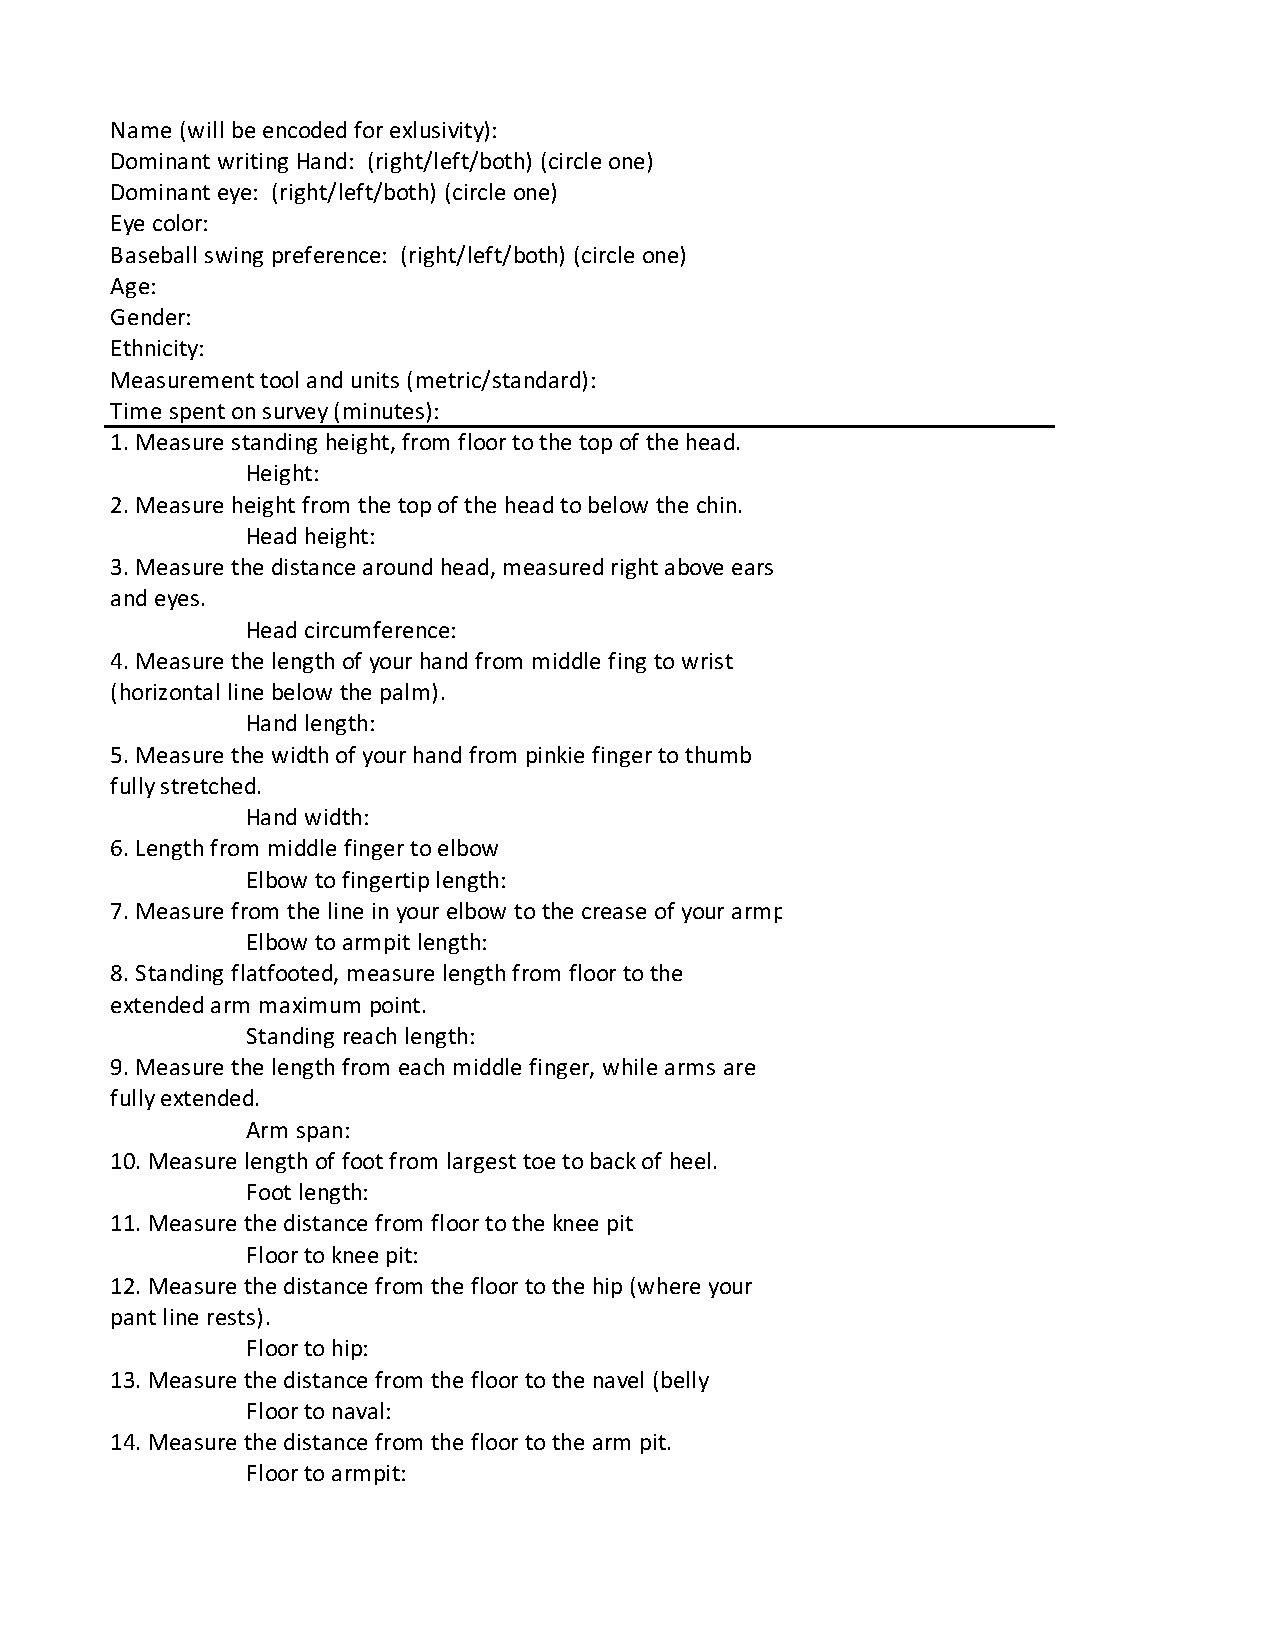
\includegraphics[trim = 0 0 0 0,clip,width=0.85\textwidth]{pdfs/project-measure-handout.pdf} }
    \end{center}
    \label{fig:handout-1}
    \hrule
\end{figure}

\newpage

\subsection{Creating Work Environment}
\label{sec:appendix-setup}

\begin{Shaded}
\begin{Highlighting}[]
\CommentTok{# Get measure data}
\CommentTok{# }
\NormalTok{measure =}\StringTok{ }\NormalTok{utils}\OperatorTok{::}\KeywordTok{read.csv}\NormalTok{( }\KeywordTok{paste0}\NormalTok{(path.to.secret, }\StringTok{"measure-students.txt"}\NormalTok{), }
                           \DataTypeTok{header=}\OtherTok{TRUE}\NormalTok{, }\DataTypeTok{quote=}\StringTok{""}\NormalTok{, }\DataTypeTok{sep=}\StringTok{"|"}\NormalTok{);}

\NormalTok{getOne =}\StringTok{ }\KeywordTok{c}\NormalTok{(}\StringTok{"hand.length"}\NormalTok{, }\StringTok{"hand.width"}\NormalTok{, }\StringTok{"arm.reach"}\NormalTok{);}
\NormalTok{measure.X =}\StringTok{ }\KeywordTok{prepare.measure.data}\NormalTok{(measure, }
                                 \DataTypeTok{getOne =}\NormalTok{ getOne)}

\CommentTok{# Get NBA data}
\CommentTok{# }
\NormalTok{nba <-}\StringTok{ }\KeywordTok{read_labelled_xlsx}\NormalTok{(}\DataTypeTok{filename =} \StringTok{"/Users/harrisonfuller/OneDrive - Washington State University (email.wsu.edu)/Classes/STATS 419/WSU_STATS419_FALL2020/datasets/NBA.xlsx"}\NormalTok{, }
                          \DataTypeTok{data_sheet =} \StringTok{"NBA Draft"}\NormalTok{);}

\NormalTok{nba.X <-}\StringTok{ }\KeywordTok{clean.nba.data}\NormalTok{(nba);}
\end{Highlighting}
\end{Shaded}

\begin{verbatim}
## Warning in FUN(X[[i]], ...): NAs introduced by coercion

## Warning in FUN(X[[i]], ...): NAs introduced by coercion
\end{verbatim}

\begin{verbatim}
## Warning: Expected 2 pieces. Additional pieces discarded in 232 rows [1, 2, 3, 4,
## 5, 6, 7, 8, 9, 10, 11, 12, 13, 14, 15, 16, 17, 18, 19, 20, ...].

## Warning: Expected 2 pieces. Additional pieces discarded in 232 rows [1, 2, 3, 4,
## 5, 6, 7, 8, 9, 10, 11, 12, 13, 14, 15, 16, 17, 18, 19, 20, ...].

## Warning: Expected 2 pieces. Additional pieces discarded in 232 rows [1, 2, 3, 4,
## 5, 6, 7, 8, 9, 10, 11, 12, 13, 14, 15, 16, 17, 18, 19, 20, ...].
\end{verbatim}

\subsubsection{Scaling Measurements}
\label{sec:appendix-scaling}

\begin{Shaded}
\begin{Highlighting}[]
\NormalTok{measure.X.nba =}\StringTok{ }\KeywordTok{prepare.measure.for.nba.comparison}\NormalTok{(}\DataTypeTok{measure.X =}\NormalTok{ measure.X, }\DataTypeTok{zmin =} \DecValTok{-3}\NormalTok{, }\DataTypeTok{zmax =} \DecValTok{3}\NormalTok{)}

\CommentTok{# compare body measurements to height}
\CommentTok{# }
\NormalTok{measure.height.Xs <-}\StringTok{ }\KeywordTok{na.omit}\NormalTok{(measure.X.nba) }\OperatorTok
\StringTok{  }\KeywordTok{mutate}\NormalTok{(}\KeywordTok{across}\NormalTok{(}\KeywordTok{c}\NormalTok{(hand.length}\OperatorTok{:}\NormalTok{wingspan), }\OperatorTok{~}\StringTok{  }\KeywordTok{round}\NormalTok{(.}\OperatorTok{/}\NormalTok{height, }\DataTypeTok{digits =} \DecValTok{2}\NormalTok{)));}

\CommentTok{# Compare body measurements to height}
\CommentTok{# }
\NormalTok{nba.height.Xs <-}\StringTok{ }\KeywordTok{na.omit}\NormalTok{(nba.X) }\OperatorTok
\StringTok{  }\KeywordTok{mutate}\NormalTok{(}\KeywordTok{across}\NormalTok{(}\KeywordTok{c}\NormalTok{(hand.length}\OperatorTok{:}\NormalTok{wingspan), }\OperatorTok{~}\StringTok{  }\KeywordTok{round}\NormalTok{(.}\OperatorTok{/}\NormalTok{height, }\DataTypeTok{digits =} \DecValTok{2}\NormalTok{)));}

\CommentTok{# merge data}
\CommentTok{# }
\NormalTok{height.prop.bind.Xs <-}\StringTok{ }\KeywordTok{rbind}\NormalTok{(nba.height.Xs, measure.height.Xs);}


\NormalTok{height.prop.merge.Xs <-}\StringTok{ }\NormalTok{height.prop.bind.Xs }\OperatorTok\StringTok{ }\KeywordTok{select}\NormalTok{(}\OperatorTok{-}\NormalTok{height) }\OperatorTok
\StringTok{  }\KeywordTok{melt}\NormalTok{(.,}\KeywordTok{c}\NormalTok{(}\DecValTok{1}\OperatorTok{:}\DecValTok{3}\NormalTok{));}
\end{Highlighting}
\end{Shaded}

\subsection{Images}
\label{sec:appendix-Images}

\begin{figure}
\centering
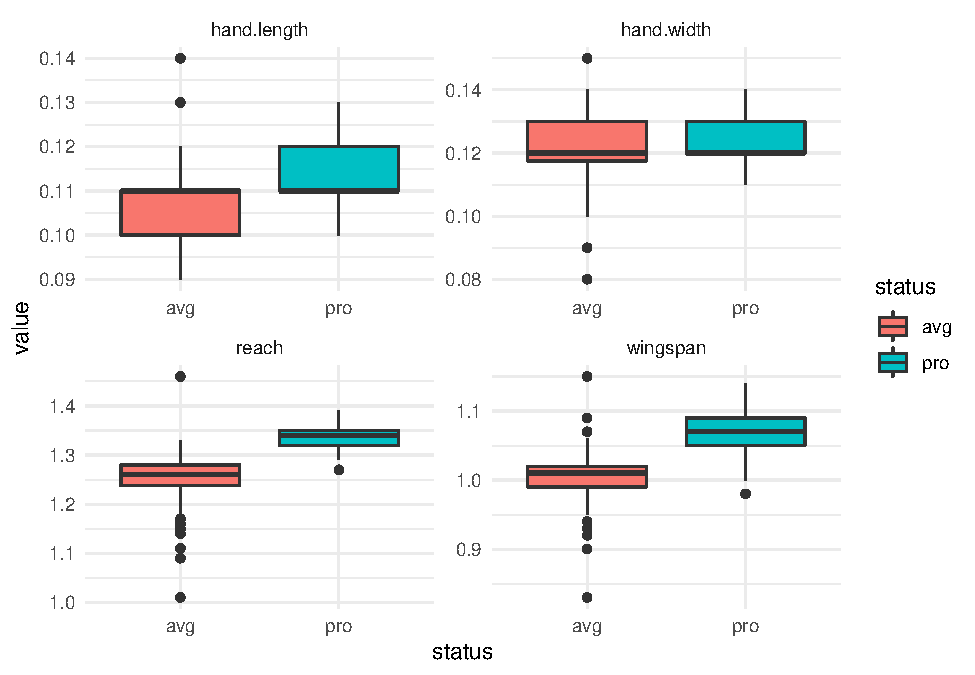
\includegraphics{project-measure-writeup_files/figure-latex/image-proportion-comparison-1.pdf}
\caption{Distribution of average participant data vs professional
basketball player data by feature. All values are subjected to anchored
scaling to height.}
\end{figure}

\begin{figure}
\centering
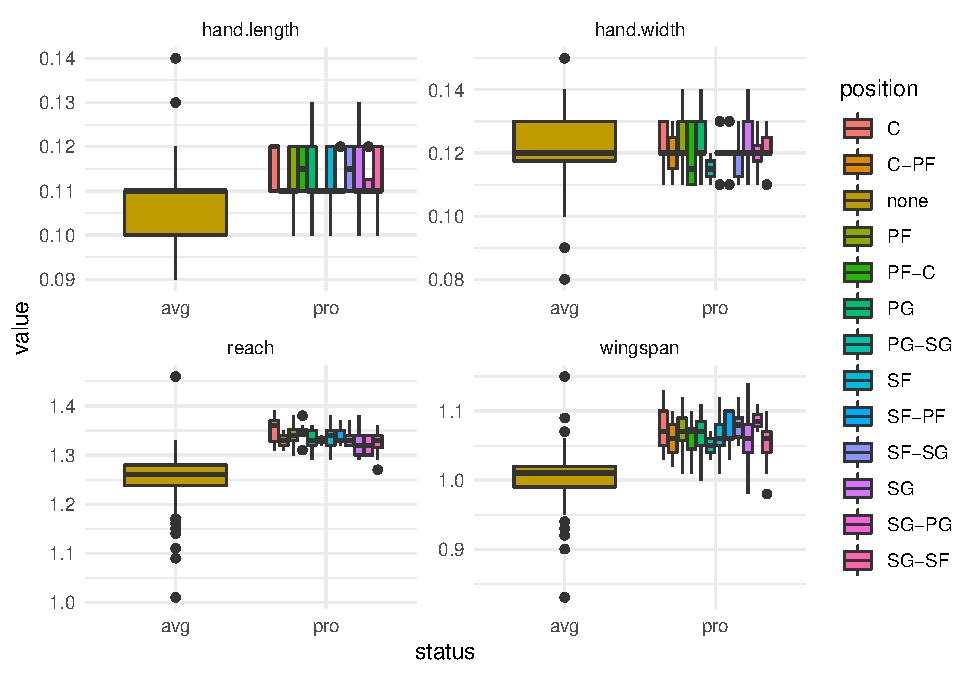
\includegraphics{project-measure-writeup_files/figure-latex/appendix-boxplot-1.pdf}
\caption{Distribution of average participant data vs professional
basketball player data by feature and position. All values are subjected
to anchored scaling to height.}
\end{figure}

\begin{figure}
\centering
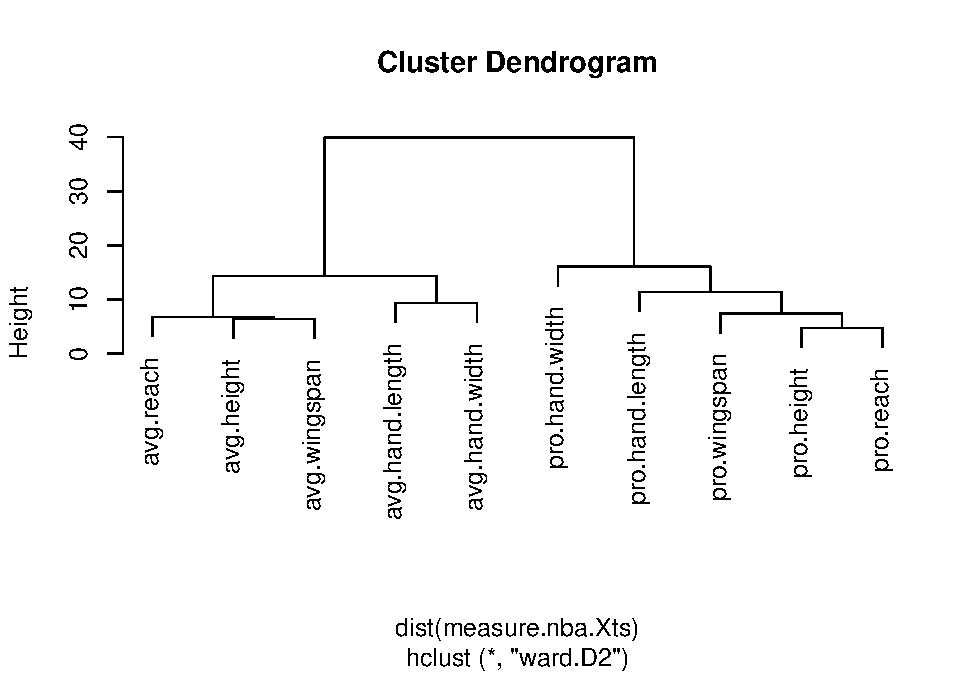
\includegraphics{project-measure-writeup_files/figure-latex/appendix-cluster-analysis-1.pdf}
\caption{Heirarchal clustering of average participant data vs
professional basketball player data by feature. All values are subjected
to anchored scaling to height.}
\end{figure}




%% appendices go here!


\newpage
\theendnotes

%%%%%%%%%%%%%%%%%%%%%%%%%%%%%%%%%%%  biblio %%%%%%%%
\newpage
\begin{auxmulticols}{2}
\singlespacing 
\bibliography{./../biblio/master.bib}

%%%%%%%%%%%%%%%%%%%%%%%%%%%%%%%%%%%  biblio %%%%%%%%
\end{auxmulticols}

\newpage
{
\hypersetup{linkcolor=black}
\setcounter{tocdepth}{3}
\tableofcontents
}



\end{document}